% A simple Tree
% Author: Stefan Kottwitz
% https://www.packtpub.com/hardware-and-creative/latex-cookbook
\documentclass[border=10pt]{standalone}
\usepackage{tikz}
\begin{document}
\tikzset{edge from parent/.append style={->,>=latex,red}}
\tikzset{level distance=60pt}
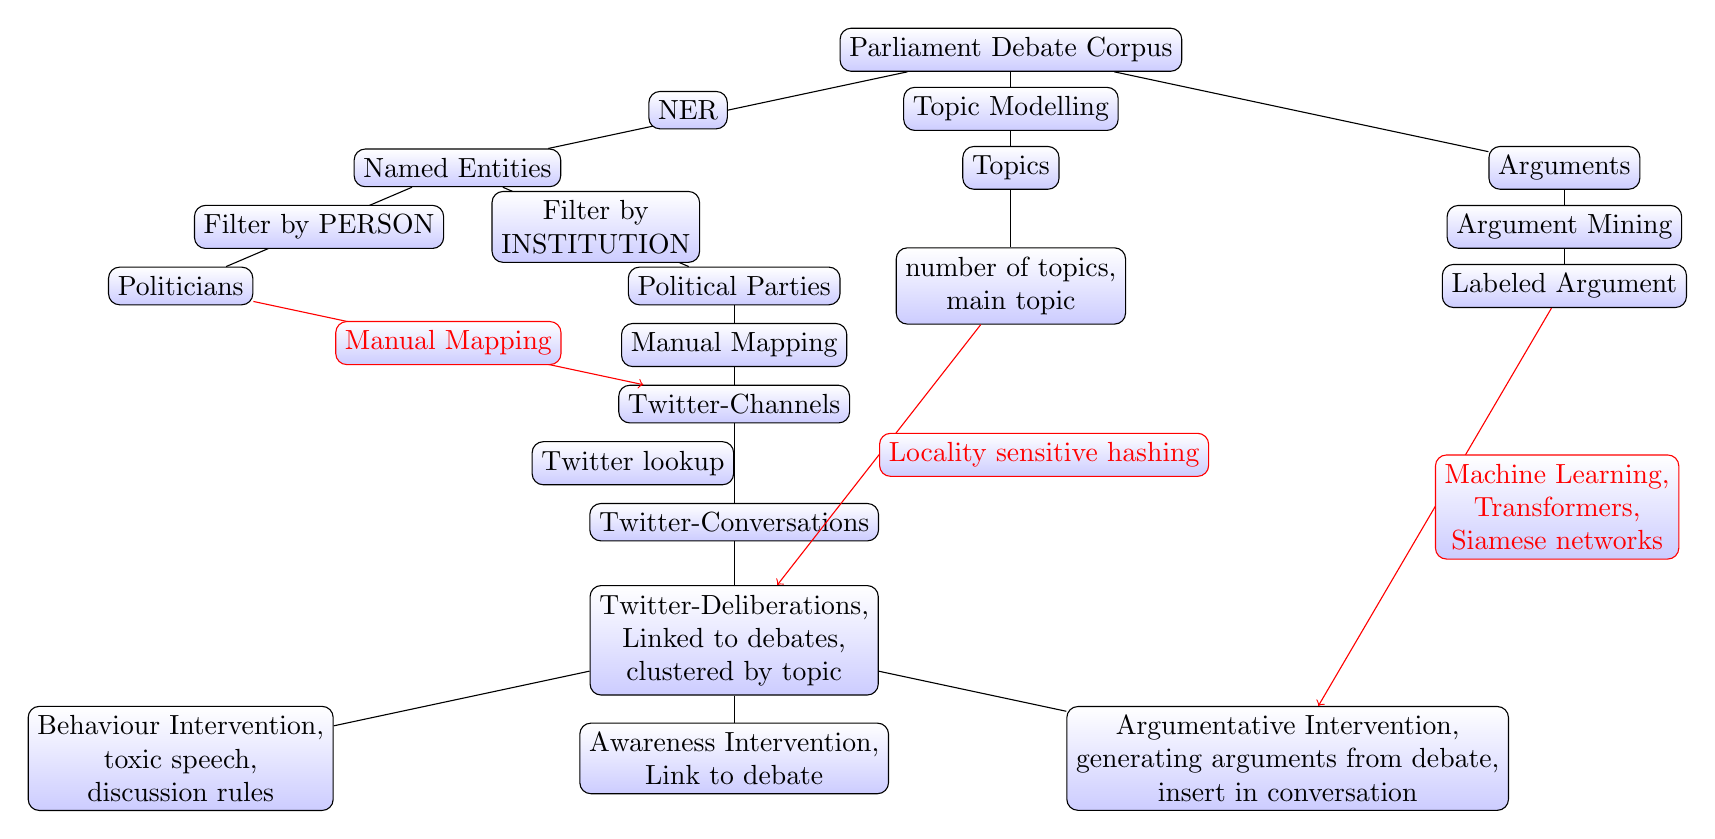
\begin{tikzpicture}[
sibling distance=20em, 
  every node/.style = {shape=rectangle, rounded corners,
    draw, align=center,
    top color=white, bottom color=blue!20}]]
  \node {Parliament Debate Corpus}
    child { node {Named Entities} 
    	child {node (p) {Politicians}    		
    		edge from parent node{Filter by PERSON}
    		}
    	child {node {Political Parties}    		
    		child {node (t) {Twitter-Channels}
    			child {node (c) {Twitter-Conversations}
    				child {node (d) {Twitter-Deliberations, \\ Linked to debates, \\clustered by topic}
						child {node (i1) {Behaviour Intervention,\\toxic speech, \\discussion rules}}
						child {node (i2) {Awareness Intervention,\\Link to debate}}		    				
						child {node (i3) {Argumentative Intervention,\\generating arguments from debate,\\insert in conversation}}		    				
    				}    					
    			edge from parent node[left]{Twitter lookup}    				
    			}
    		edge from parent node{Manual Mapping}
    		}
    	edge from parent node{Filter by \\ INSTITUTION}
    	}
    edge from parent node[left]{NER}    		
    }
    child { node {Topics}      
      child { node(k) {number of topics,\\main topic}
      		}
      edge from parent node{Topic Modelling} 
      }
    child { node {Arguments} 
    	child {node  (debate_args) {Labeled Argument}    		
    	edge from parent node{Argument Mining}
    		}
    }    
    ;     
    \draw[red,->] (p) -- (t) node[midway]{Manual Mapping};
    \draw[red,->] (k) -- (d) node[midway, right]{Locality sensitive hashing};
    \draw[red,->] (debate_args) -- (i3) node[midway, right]{Machine Learning, \\Transformers,\\ Siamese networks};
\end{tikzpicture}
\end{document}